\documentclass[a4paper,10pt]{report}
\usepackage[utf8]{inputenc}
\usepackage{hyperref}
\usepackage{graphicx}

\setlength{\parindent}{0mm}
\setlength{\parskip}{2mm}
\setlength{\textwidth}{450pt} %Veränderung des Textblocks in Anpassung an den R Zeilenüberhang bei Aufrufswiederholungen
\setlength{\hoffset}{-50pt} % "
\setlength{\topmargin}{-30pt}
\setlength{\textheight}{670pt}

% Title Page
\title{BRAKER2 Userguide}
\author{Katharina J.~Hoff}


\begin{document}
\maketitle

\tableofcontents

\chapter{Introduction}

\section{What is BRAKER2?}

The rapidly growing number of sequenced genomes requires fully automated methods for accurate gene structure annotation. With this goal in mind, we have developed BRAKER1 \cite{braker1}, a combination of GeneMark-ET \cite{GeneMark-ET} and AUGUSTUS \cite{AUGUSTUS}, that uses genomic and RNA-Seq data to automatically generate full gene structure annotations in novel genomes.

However, the quality of RNA-Seq data that is available for annotating a novel genome is variable, and in some cases, RNA-Seq data is not available, at all.

BRAKER2 is an extension of BRAKER1 which allows for \textbf{fully automated training} of the gene prediction tools GeneMark-EX \cite{GeneMark-EX} and AUGUSTUS from RNA-Seq and/or protein homology information, and that integrates the extrinsic evidence from RNA-Seq and protein homology information into the \textbf{prediction}.

In contrast to other available methods that rely on protein homology information, BRAKER2 reaches high gene prediction accuracy even in the absence of the annotation of very closely related species and in the absence of RNA-Seq data. 

BRAKER2 can also combine RNA-Seq and protein homology information.

\section{Keys to successful gene prediction}

\begin{itemize}
 \item In order to predict genes accurately in a novel genome, the genome should be masked for repeats. This will avoid the prediction of false positive gene structures in repetitive and low complexitiy regions. Repeat masking is also essential for mapping RNA-Seq data to a genome. In case of GeneMark-EX and AUGUSTUS, softmasking (i.e.~putting repeat regions into lower case letters and all other regions into upper case letters) leads to better results than hardmasking (i.e.~replacing letters in repetitive regions by the letter \texttt{N} for unknown nucleotide).
 
 \item Many genomes have gene structures that will be predicted accurately with standard parameters of GeneMark-ET and AUGUSTUS within BRAKER2. However, some genomes have clade-specific features, i.e.~special branch point model in fungi, or non-standard splice-site patterns. Please read the options section \ref{options} in order to determine whether any of the custom options may improve gene prediction accuracy in the genome of your target species.
\end{itemize}

\section{Overview of modes for running BRAKER2}

BRAKER2 mainly features semi-unsupervised, extrinsic evidence data (RNA-Seq or protein spliced alignment information) supported training of GeneMark-EX and subsequent training of AUGUSTUS with integration of extrinsic evidence in the final gene prediction step. However, there are now a number of additional pipelines included in BRAKER2. In the following, we give an overview:

\begin{itemize}
 \item genome and RNA-Seq file from the same species (see figure \ref{braker-main}A); this approach is suitable for RNA-Seq libraries with a good coverage of the transcriptome,
 \item genome file and database of proteins that may be of longer evolutionary distance to the target species (see figure \ref{braker-main}B; this approach is suitable if no RNA-Seq data is available, and if not protein data from a very closely related species is available,
 \item genome file and file with proteins of short evolutionary distance (see figure \ref{braker2-sidetrack}D); this approach is suitable if RNA-Seq data is not available and if the reference species is very closely related,
 \item genome and RNA-Seq file and proteins for short evolutionary distance (see figures \ref{braker2-sidetrack}C and \ref{braker2-sidetrack}E). In both cases, GeneMark-ET is trained supported by RNA-Seq data, and the resulting gene predictions are used for training AUGUSTUS. In approach C), protein alignment information is used in the gene prediction step with AUGUSTUS, only. In approach E), protein spliced alignment data is used to complement the training set for AUGUSTUS. The latter approach is in particular suitable if RNA-Seq data does not produce a sufficiently high number of training gene structures for AUGUSTUS, and if a very closely related and already annotated species is available.
\end{itemize}

\begin{figure}
\begin{center}
\begin{tabular}{c c c c }
 A) & 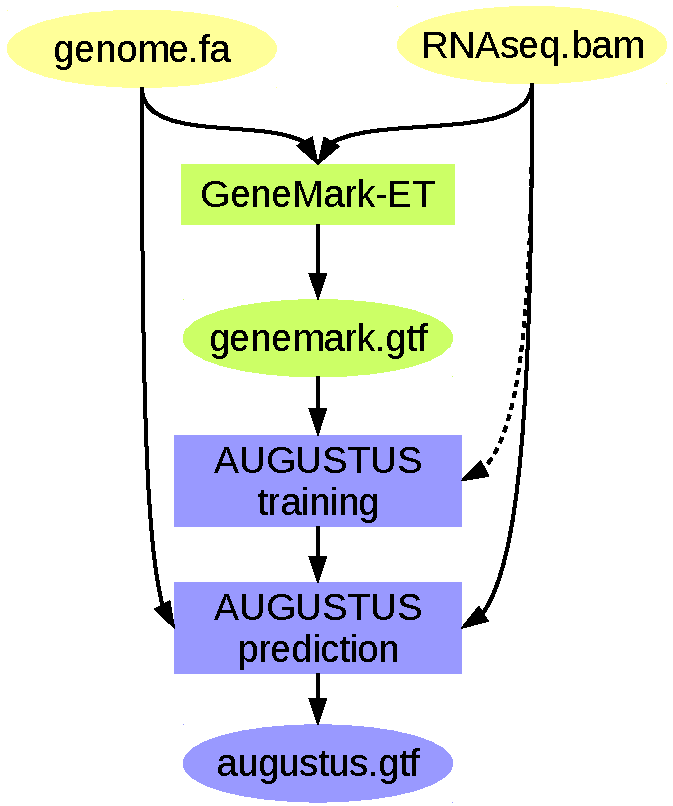
\includegraphics[scale=0.4]{./figs/braker1.pdf} & B) &  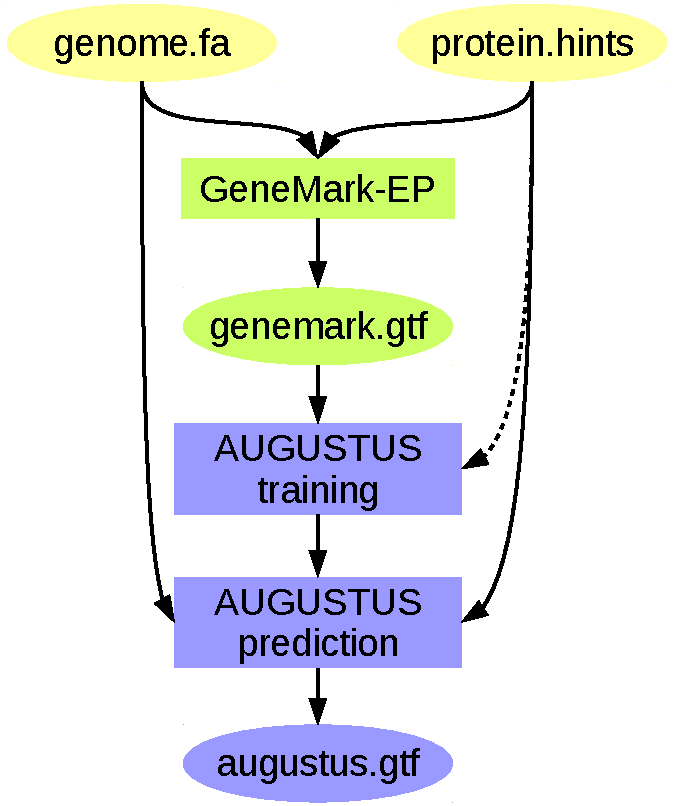
\includegraphics[scale=0.4]{./figs/braker2_ep.pdf}\\
 % braker1.pdf: 323x387 pixel, 72dpi, 11.39x13.65 cm, bb=0 0 323 387
 \end{tabular}
 \caption{BRAKER2 pipeline A) training GeneMark-ET supported by RNA-Seq spliced alignment information, prediction with AUGUSTUS with that same spliced alignment information, B) training GeneMark-EP on protein spliced alignment information, prediction with AUGUSTUS with that same spliced alignment information. Proteins used for B) can be of longer evolutionary distance.\label{braker-main}}
 \end{center}
 \end{figure}

\begin{figure}
\begin{center}
\begin{tabular}{c c c c c c}
 C) & 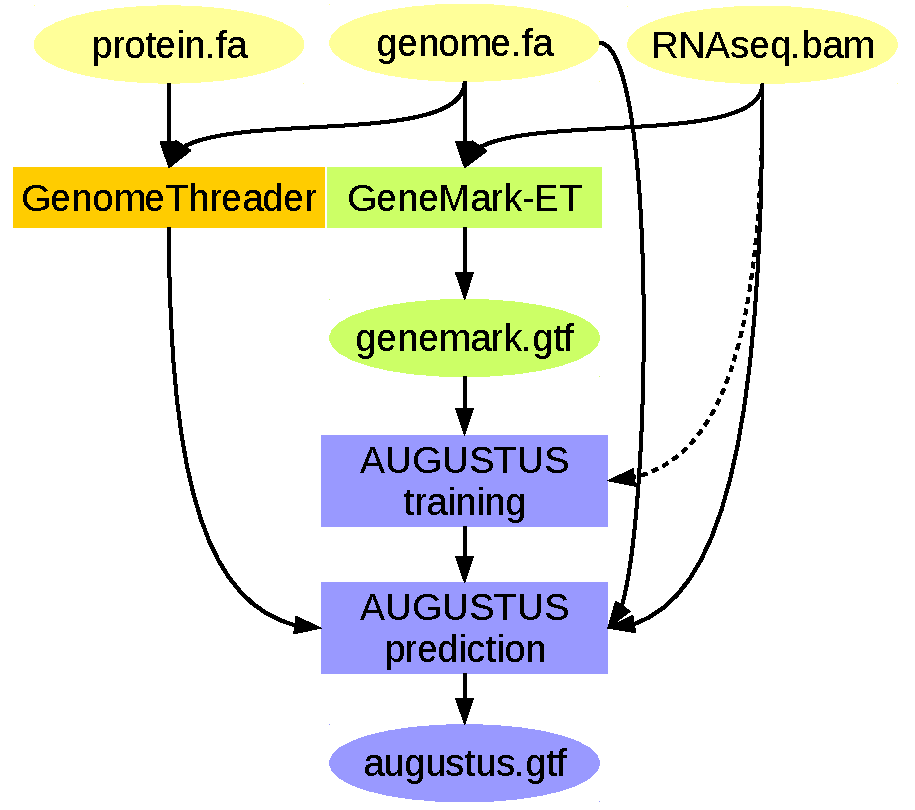
\includegraphics[scale=0.27]{./figs/braker2.pdf} & D) &  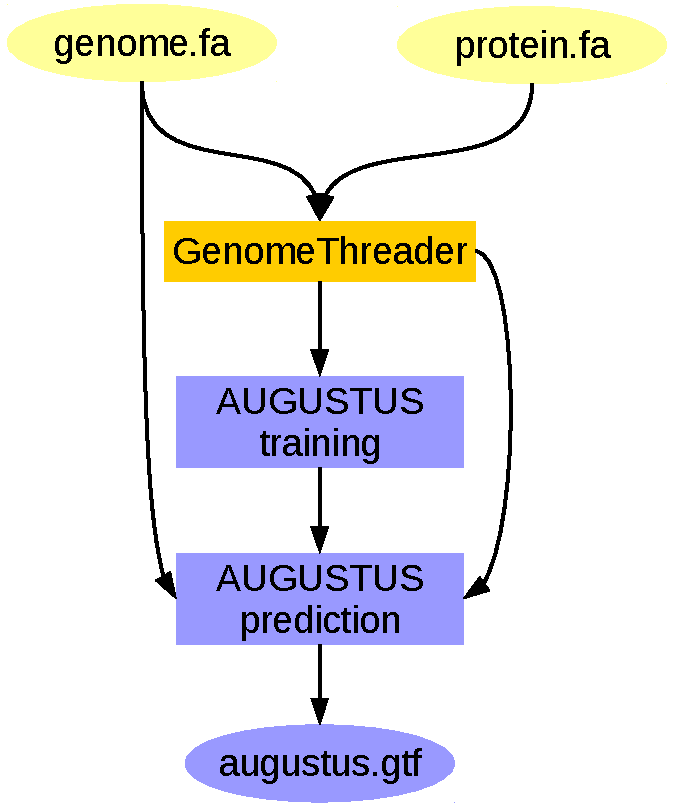
\includegraphics[scale=0.27]{./figs/braker2_gth.pdf} & E) & 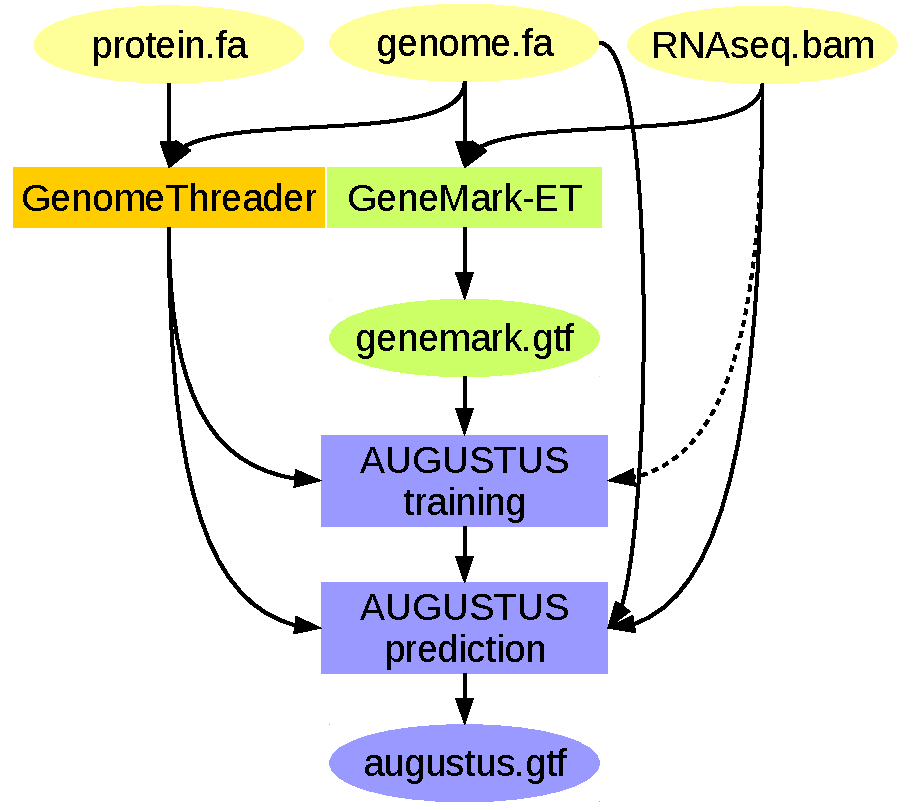
\includegraphics[scale=0.27]{./figs/braker2_train_from_both.pdf}\\
 % braker1.pdf: 323x387 pixel, 72dpi, 11.39x13.65 cm, bb=0 0 323 387
 \end{tabular}
 \caption{BRAKER2 pipeline C) training GeneMark-ET supported by RNA-Seq spliced alignment information, prediction with AUGUSTUS with spliced alignment information from RNA-Seq data and with gene features determined by alignments from proteins of a very closely related species against the target genome, D) training AUGUSTUS on the basis of spliced alignment information from proteins of a very closely related species against the target genome, E) training GeneMark-ET on the basis of RNA-Seq spliced alignment information, training AUGUSTUS on a set of training gene structures compiled from RNA-Seq supported gene structures predicted by GeneMark-ET and spliced alignment of proteins of a very closely related species.\label{braker2-sidetrack}}
 \end{center}
 \end{figure} 
 

\chapter{Installation}

\section{Supported software versions}

At the time of release, this BRAKER2 version was tested with:

\begin{itemize}
\item AUGUSTUS 3.2.2
   \item  GeneMark-EX xxx
   \item  BAMTOOLS 2.4.1
   \item  SAMTOOLS 0.1.19-96b5f2294a
   \item  GenomeThreader 1.1.6
   \item  Spaln 2.3.1
   \item  Exonerate 2.2.0
\end{itemize}

\section{BRAKER2}

\subsection{Perl pipeline dependencies}

BRAKER2 is implemented in Perl. Running BRAKER2 requires a Linux-system with \texttt{bash} and Perl. Furthermore, BRAKER2 requires the following CPAN-Perl modules to be installed:

\begin{itemize}
 \item 		  \texttt{File::Spec::Functions}
				\item \texttt{Hash::Merge}
				\item \texttt{List::Util}
				\item \texttt{Logger::Simple}
				\item \texttt{Module::Load::Conditional}
				\item \texttt{Parallel::ForkManager}
				\item \texttt{POSIX}
				\item \texttt{Scalar::Util::Numeric}
				\item \texttt{YAML}
\end{itemize}

   	On Ubuntu, for example, install the modules with CPANminus: \texttt{cpanm [Module::Name]}.

   BRAKER2 also uses a Perl module \texttt{helpMod.pm} that is not available on CPAN. This module is 
   part of the BRAKER2 relase and does not require separate installation.  

\subsection{BRAKER2 components} \label{Executability}

BRAKER2 is a collection of Perl scripts and a Perl module. The main script that will be called in order to run BRAKER2 is \texttt{braker.pl}. Additional Perl components are:

\begin{itemize}
\item \texttt{align2hints.pl}
\item \texttt{filterGenemark.pl}
\item \texttt{filterIntronsFindStrand.pl}
\item \texttt{startAlign.pl}
\item \texttt{helpMod.pm}
\end{itemize}

All Perl scripts (files ending with \texttt{*.pl}) that are part of BRAKER2 must be executable in order to run BRAKER2. This should already be the case if you download BRAKER2 from our website. Executability may be overwritten if you e.g.~transfer BRAKER2 on a USB-stick to anothre computer. In order to check whether required files are executable, run the following command in the directory that contains BRAKER2 Perl scripts:

\begin{verbatim}
ls -l *.pl
\end{verbatim}

The output should be similar to this:

\begin{verbatim}
-rwxr-xr-x 1 braker braker  13802 Jan 12 14:23 align2hints.pl
-rwxr-xr-x 1 braker braker 159944 Jan 16 16:42 braker.pl
-rwxr-xr-x 1 braker braker  21217 Jul  3  2017 filterGenemark.pl
-rwxr-xr-x 1 braker braker   5716 Jul 12  2017 filterIntronsFindStrand.pl
-rwxr-xr-x 1 braker braker  32123 Jan 12 14:23 startAlign.pl
\end{verbatim}

It is important that the \texttt{x} in \texttt{-rwxr-xr-x} is present for each script. If that is not the case, run

\begin{verbatim}
chmod a+x *.pl
\end{verbatim}

in order to change file attributes.

You may find it helpful to add the directory in which BRAKER2 perl scripts reside to 
    your \texttt{\$PATH} environment variable. For a single bash session, enter:

    \begin{verbatim}
    PATH=/your_path_to_braker/:$PATH
    export PATH
    \end{verbatim}
    
To make this PATH modification available to all bash sessions, add the above lines to a startup script (e.g.\texttt{$sim$/.bashrc}).

\section{Bioinformatics software dependencies}

BRAKER2 calls upon various bioinformatics software tools that are not part of BRAKER2. Some tools are obligatory, i.e.~BRAKER2 will not run at all if these tools are not present on your system. Other tools are optional. Please install all tools that are required for running BRAKER2 in the mode of your choice.

\subsection{Mandatory tools}

\subsubsection{GeneMark-EX}

Download GeneMark-EX from \url{http://exon.gatech.edu/GeneMark/license_download.cgi}.
 Unpack and install GeneMark-EX as described in GeneMark-EX's \texttt{README} file.

BRAKER2 can find GeneMark-EX executables either by locating them in an environment variable \texttt{GENEMARK\_PATH}, or by taking a command line argument\\ (\texttt{--GENEMARK\_PATH=/your\_path\_to\_GeneMark-EX/gmes\_petap/}). In order to set the environment variable for your current Bash session, type: 

    \begin{verbatim}
    export GENEMARK_PATH=/your_path_to_GeneMark-ET/gmes_petap/
\end{verbatim}

Add the above lines to a startup script (e.g.~\texttt{$\sim$/.bashrc}) in order to make it available to all bash sessions.

\subsubsection{AUGUSTUS}

Download AUGUSTUS from \url{http://bioinf.uni-greifswald.de/augustus/downloads/index.php}.
 Unpack AUGUSTUS and install AUGUSTUS  according to AUGUSTUS \texttt{README.TXT}. 
 
 AUGUSTUS comes with pre-compiled binaries (located in the 
   \texttt{augustus-x.x.x/bin} folder). However, you should compile AUGUSTUS on your own system in order to avoid problems with versions of libraries used by AUGUSTUS. Compilation instructions are provided in the AUGUSTUS \texttt{README.TXT} file
   (\texttt{augustus-x.x.x/README.txt}).

AUGUSTUS consists of \texttt{augustus}, the gene prediction tool, additional C++ tools located in\\ \texttt{augustus/auxprogs} and Perl scripts located in \texttt{augustus/scripts}. Perl scripts must be executable (see instructions in section \ref{Executability} on page \pageref{Executability}). 
   
   The C++ tool \texttt{bam2hints} is an essential component of BRAKER2. Sources are located in \\\texttt{augustus-x.x.x/auxprogs/bam2hints}. Make sure that you compile \texttt{bam2hints} on your system (it should be automatically compiled when AUGUSTUS is compiled, but in case of problems with \texttt{bam2hints}, please read troubleshooting instructions in 
   \texttt{augustus-x.x.x/auxprogs/bam2hints/README}).
   
   Since BRAKER2 is a pipeline that trains AUGUSTUS, i.e.~writes species specific parameter files, BRAKER2 needs writing access to the configuration directory of AUGUSTUS that contains such files  (\texttt{augustus-x.x.x/config/}). If you install AUGUSTUS
   globally on your system, the \texttt{config} folder will typically not be writable by all users. Either make the directory where \texttt{config} resides recursively writable to users of AUGUSTUS, or copy the \texttt{config/} folder (recursively) to a location where users have writing permission. 
   
   AUGUSTUS will locate the \texttt{config} folder by looking for an environment variable \texttt{\$AUGUSTUS\_CONFIG\_PATH}. If the \texttt{\$AUGUSTUS\_CONFIG\_PATH} environment variable is not set, then BRAKER2 will look in 
    the path \texttt{../config} relative to the directory in which it finds an AUGUSTUS executable. Alternatively, you can supply the variable as a command line argument to BRAKER2\\ (\texttt{--AUGUSTUS\_CONFIG\_PATH=/your\_path\_to\_AUGUSTUS/augustus/config/}). We recommend that you export the variable e.g.~for your current bash session:

    \begin{verbatim}
    export AUGUSTUS_CONFIG_PATH=/your_path_to_AUGUSTUS/augustus/config/
    \end{verbatim}

In order to make the variable available to all Bash sessions, add the above line to a startup script, e.g.~\texttt{$\sim$/.bashrc}.
   
   \paragraph{Modification of \texttt{\$PATH}.} Adding adding directories of AUGUSTUS binaries and scripts to your \texttt{\$PATH} variable enables your system to locate these tools, automatically. It is not a requirement for running BRAKER2 to do this, because BRAKER2 will try to guess them from the location of another environment variable (\texttt{\$AUGUSTUS\_CONFIG\_PATH}), or both directories can be supplied as command line arguments to \texttt{braker.pl}, but we recommend to add them to your \texttt{\$PATH} variable. For your current bash session, type:

    \begin{verbatim}
    PATH=:/your_path_to_augustus/bin/:/your_path_to_augustus/scripts/:$PATH
    export PATH
    \end{verbatim}

    For all your BASH sessions, add the above lines to a startup script (e.g.\texttt{$sim$/.bashrc}).

   

\subsubsection{Bamtools}

Download BAMTOOLS (e.g.~\texttt{git clone \url{https://github.com/pezmaster31/bamtools.git}}). Install BAMTOOLS by typing the following in your shell:\\

 \begin{verbatim}
   cd your-bamtools-directory
   mkdir build
   cd build
   cmake ..
   make
 \end{verbatim}

 BRAKER2 can locate the bamtools binary either by using an environment variable \texttt{\$BAMTOOLS\_PATH}, or by taking a command line argument (\texttt{--BAMTOOLS\_PATH=/your\_path\_to\_bamtools/bin/}). In order to set the environment variable e.g.~for your current bash session, type:

    \begin{verbatim}
        export BAMTOOLS_PATH=/your_path_to_bamtools/bin/ 
    \end{verbatim} 

    Add the above line to a startup script (e.g.~\texttt{$\sim$/.bashrc}) in order to set the environment variable for all bash sessions.
    
\subsection{Optional tools}

\subsubsection{Samtools}

Samtools is not required for running BRAKER2 if all your files are formatted, correctly (i.e.~all sequences should have short and unique fasta names). If you are not sure
      whether all your files are fomatted correctly, it might be helpful to have Samtools
      installed because BRAKER2 can automatically fix certain format issues by using Samtools. 

      As a prerequisite for Samtools, download and install \texttt{htslib} (e.g.~ 
      \texttt{git clone \url{https://github.com/samtools/htslib.git}}, follow the \texttt{htslib} documentation for 
      installation).

      Download and install Samtools (e.g. \texttt{git clone \url{git://github.com/samtools/samtools.git}}), 
      subsequently follow Samtools documentation for installation).    

      BRAKER2 can find Samtools either by taking a command line argument\\ (\texttt{--SAMTOOLS\_PATH=/your\_path\_to\_samtools/}), or by using an environment variable \texttt{\$SAMTOOLS\_PATH}. For exporting the variable, e.g.~for your current bash session, type:

    \begin{verbatim}
      export SAMTOOLS_PATH=/your_path_to_samtools/
    \end{verbatim}
    
        Add the above line to a startup script (e.g.~\texttt{$\sim$/.bashrc}) in order to set the environment variable for all bash sessions.
\subsubsection{GenomeThreader}

This tool is required, only, if you would like to run protein to genome alignments with BRAKER2 using GenomeThreader. This is a suitable approach if an annotated species of short evolutionary distance to your target genome is available. Download GenomeThreader from \url{http://genomethreader.org/}. Unpack and install according to \texttt{gth/README}.

\subsubsection{Spaln}

This tool is required, only, if you would like to run protein to genome alignments with BRAKER2 using Spaln. This is a suitable approach if an annotated species of short evolutionary distance to your target genome is available. (We recommend the usage of GenomeThreader instad of Spaln.) Download Spaln from \url{http://www.genome.ist.i.kyoto-u.ac.jp/~aln_user}. Unpack and install according to \texttt{spaln/doc/SpalnReadMe22.pdf}.

\subsubsection{Exonerate}

This tool is required, only, if you would like to run protein to genome alignments with BRAKER2 using Exonerate. This is a suitable approach if an annotated species of short evolutionary distance to your target genome is available. (We recommend the usage of GenomeThreader instad of Exonerate because Exonerate is comparably slower and has lower specificity than GenomeThreader.) Download Exonerate from \url{https://github.com/nathanweeks/exonerate}. Unpack and install according to \texttt{exonerate/README}. (On Ubuntu, download and install by typing  \texttt{sudo apt-get install exonerate}.)

\chapter{Running BRAKER2}


\begin{itemize}
 \item genome and RNA-Seq file and proteins for short evolutionary distance (see figures \ref{braker2-sidetrack}C and \ref{braker2-sidetrack}E). In both cases, GeneMark-ET is trained supported by RNA-Seq data, and the resulting gene predictions are used for training AUGUSTUS. In approach C), protein alignment information is used in the gene prediction step with AUGUSTUS, only. In approach E), protein spliced alignment data is used to complement the training set for AUGUSTUS. The latter approach is in particular suitable if RNA-Seq data does not produce a sufficiently high number of training gene structures for AUGUSTUS, and if a very closely related and already annotated species is available.
\end{itemize}

\section{BRAKER2 with RNA-Seq data (only)}

This approach is suitable for genomes of species for which RNA-Seq libraries with a good coverage of the transcriptome are available. The pipeline is illustrated in figure \ref{braker-main}A) on page \pageref{braker-main}.

BRAKER2 can either extract RNA-Seq spliced alignment information from \texttt{bam} files, or it can use such extracted information, directly.

In order to run BRAKER2 with RNA-Seq data supplied as \texttt{bam} file(s) (in case of multiple files, separate them by comma), run:

\begin{verbatim}
   braker.pl --species=yourSpecies --genome=genome.fasta --bam=file1.bam,file2.bam
\end{verbatim}

In order to run BRAKER2 with RNA-Seq spliced alignment information that has already been extracted, run:

\begin{verbatim}
   braker.pl --species=yourSpecies --genome=genome.fasta \
      --hints=hints1.gff,hints2.gff
\end{verbatim}

The format of such a hints file must be as follows (tabulator separated file):

\begin{verbatim}
chrName	b2h	intron	6591	8003	1	+	.	pri=4;src=E
chrName	b2h	intron	6136	9084	11	+	.	mult=11;pri=4;src=E
...
\end{verbatim}

The source \texttt{b2h} in the second column and the source tag \texttt{src=E} in the last column are essential for BRAKER2 to determine whether a hint has been generated from RNA-Seq data. 

\section{BRAKER2 with proteins of longer evolutionary distance}

This approach is suitable for genomes of species for which no RNA-Seq libraries are available and for which no closely related and well annotated genome is available. A database of proteins with longer evolutionary distance to the target species may be used in this case. The pipeline is illustrated in figure \ref{gatech} on page \pageref{gatech}.

\begin{figure}
 \centering
 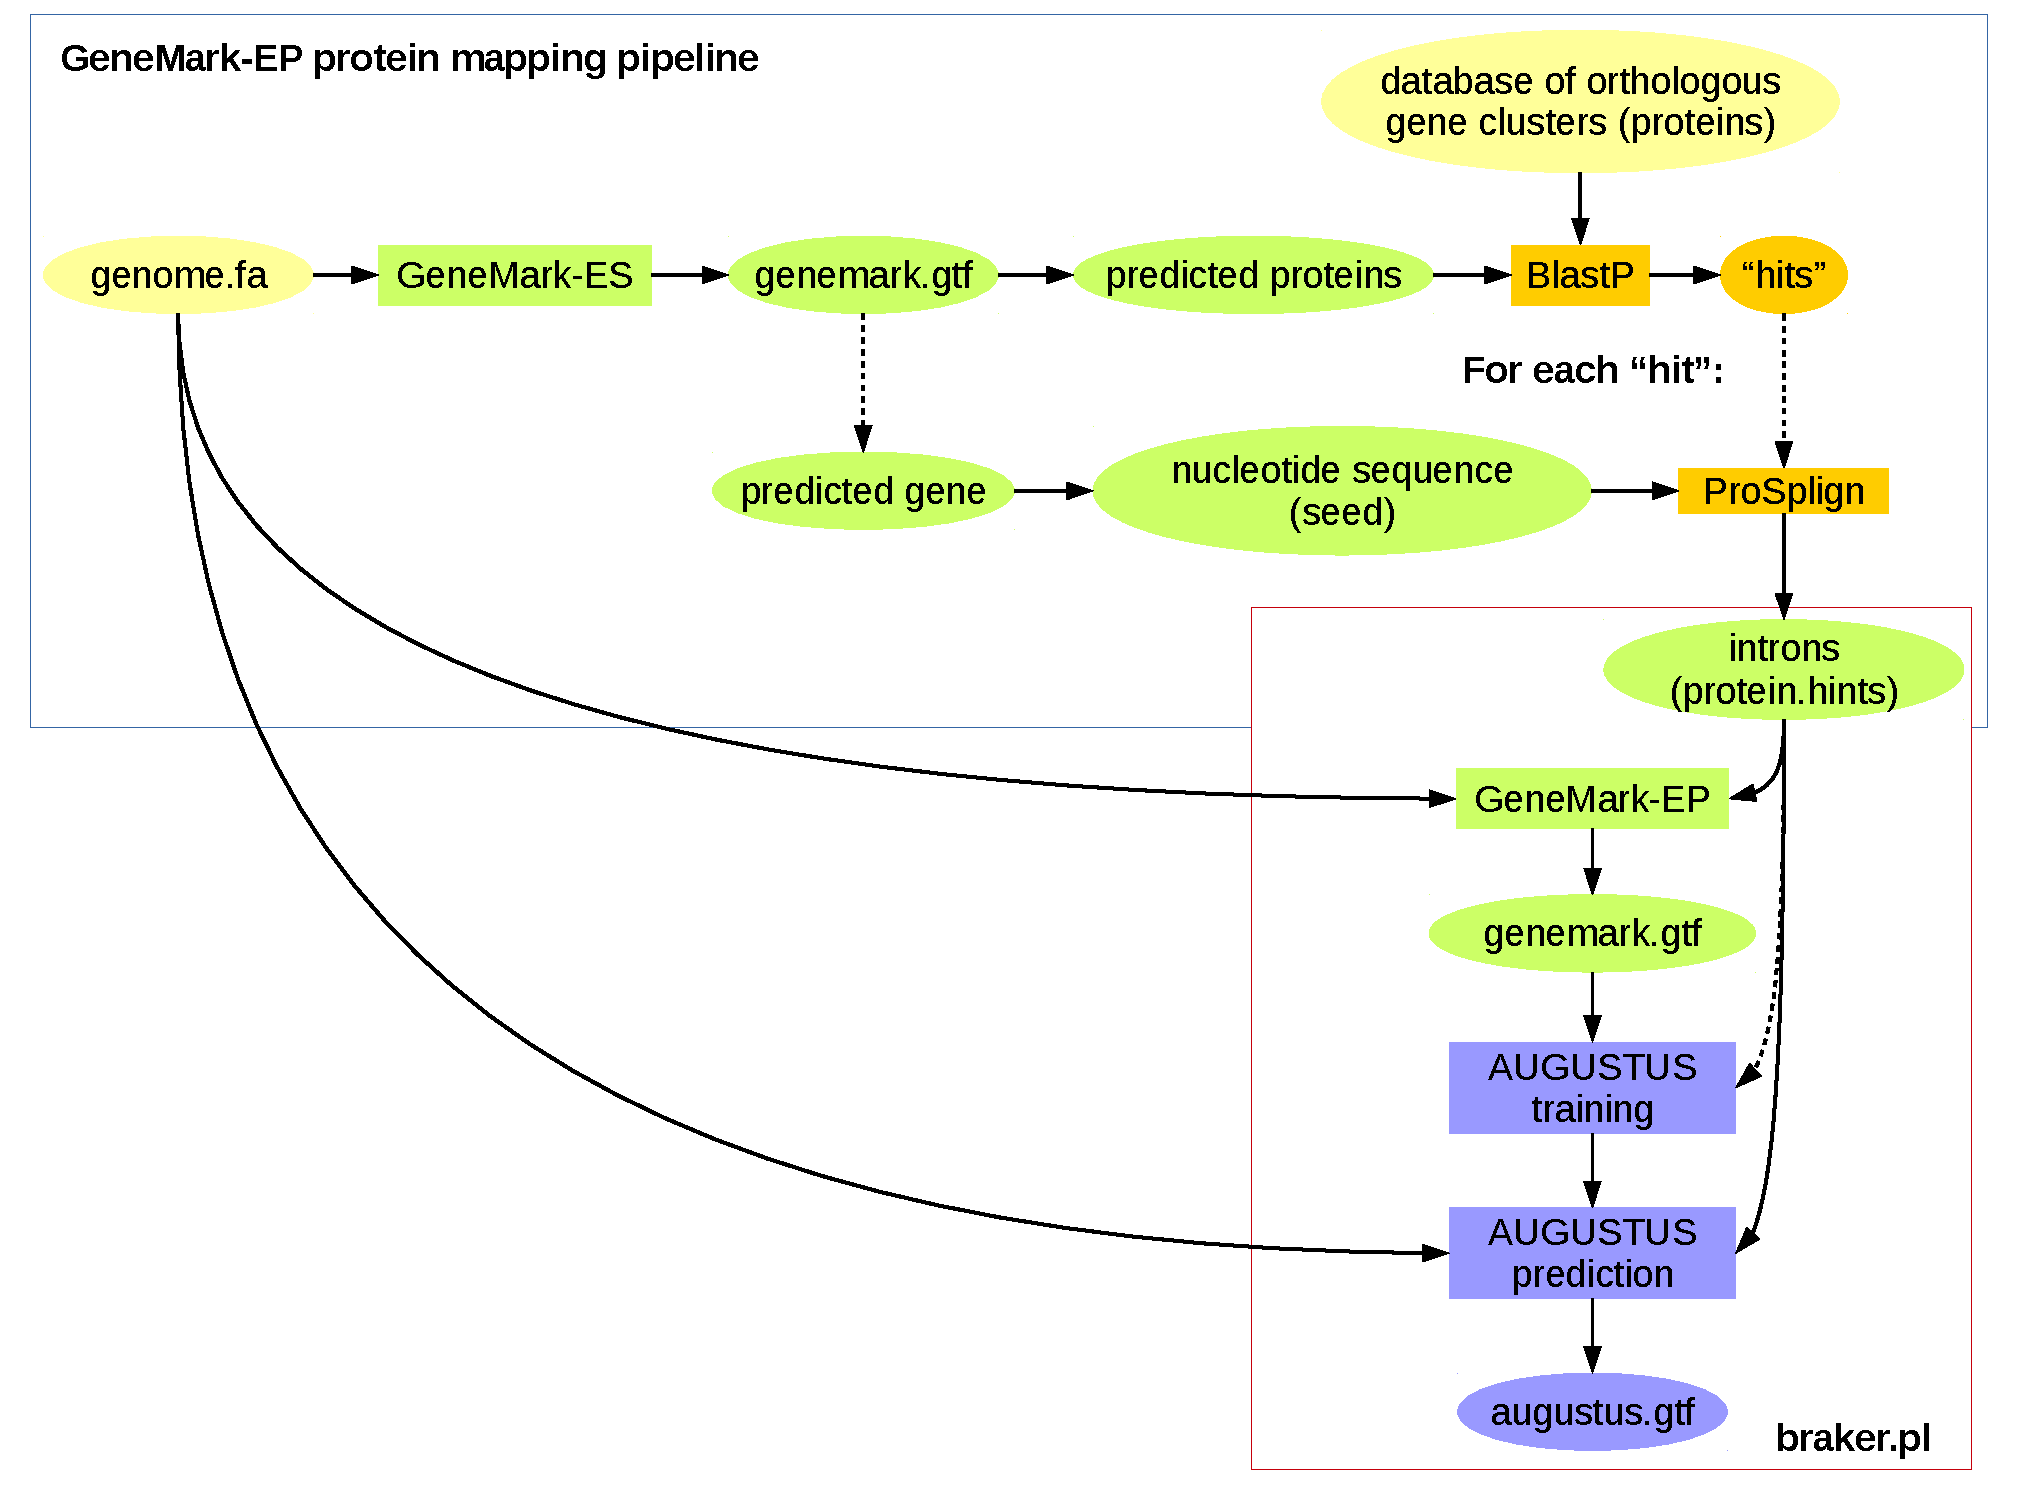
\includegraphics[scale=0.4]{./figs/gatech-prot-pipeline.pdf}
 % gatech-prot-pipeline.pdf: 972x713 pixel, 72dpi, 34.29x25.15 cm, bb=0 0 972 713
 \caption{BRAKER2 and GeneMark-EP protein mapping pipeline.}
 \label{gatech}
\end{figure}

Running BRAKER2 with proteins of longer evolutionary distance requires the preparation of ``protein hints'' before running BRAKER2, itself. Preparing protein hints is in this case not part of BRAKER2 because in contrast to BRAKER2, which can run on a work station with one or multiple cores, the GeneMark-EP specific protein mapping pipeline requires a cluster for execution.

For running BRAKER2 in this mode, type:

\begin{verbatim}
   braker.pl --species=yourSpecies --genome=genome.fasta \
      --hints=hints.gff --epmode
\end{verbatim}

The format of such a hints file must be as follows (tabulator separated file):

\begin{verbatim}
chrName	ProSplign	intron	6591	8003	5	+	.	mult=5;pri=4;src=P
chrName	ProSplign	intron	6136	9084	11	+	.	mult=11;pri=4;src=P
...
\end{verbatim}

The source \texttt{ProSplign} in the second column and the source tag \texttt{src=P} in the last column are essential for BRAKER2 to determine whether a hint has been generated from remote homology protein data. 

\section{BRAKER2 with proteins of shorter evolutionary distance}

This approach is suitable if RNA-Seq data for the species of the target genome is not available and if a well annotated and very closely related reference species is available. The pipeline is illustrated in figure \ref{braker2-sidetrack}D) on page \pageref{braker2-sidetrack}.

For running BRAKER2 in this mode, type:

\begin{verbatim}
   braker.pl --species=yourSpecies --genome=genome.fasta \
      --prot_seq=proteins.fa --prg=gth --ALIGNMENT_TOOL_PATH=/path/to/gth/binary \
      --gth2traingenes --trainFromGth
\end{verbatim}

It is possible to generate protein alignments externally, prior running BRAKER2, itself. The compatible command for running GenomeThreader prior running BRAKER2, is:

\begin{verbatim}
   gth -genomic genome.fa  -protein protein.fa -gff3out -skipalignmentout -o gth.aln
\end{verbatim}


In order to use such externally created alignment files, run:

\begin{verbatim}
   braker.pl --species=yourSpecies --genome=genome.fasta \
      --prot_aln=proteins.aln --prg=gth --gth2traingenes --trainFromGth
\end{verbatim}

It is also possible to run BRAKER2 in this mode using an already prepared hints file. In this case, run:

\begin{verbatim}
   braker.pl --species=yourSpecies --genome=genome.fasta \
      --hints=hints.gff --prg=gth --gth2traingenes --trainFromGth
\end{verbatim}

Format of the hints file should look like this:

\begin{verbatim}
 INSERT EXAMPLE!
\end{verbatim}


\section{BRAKER2 with RNA-Seq and protein data}

BRAKER2 with RNA-Seq and protein data is currently still under development. BRAKER2 currently does not train GeneMark-EX from protein and RNA-Seq data, yet. However, if RNA-Seq data of the target species and protein data of a very closely related reference species are available, BRAKER2 already supports the following to modes.

\subsection{Adding protein data of short evolutionary distance to gene prediction step}

\subsection{Extending training gene set with proteins of short evolutionary distance}

\chapter{Output of BRAKER2}

\chapter{Example data}


% 
% 
%               3. RUNNING BRAKER2
%               ------------------
% 
% BRAKER2 has two mandatory arguments: a genome file in fasta format and one file containing 
% information on RNA-Seq alignments to that genome file (either in bam format or in AUGUSTUS hints 
% format).
% 
% The genome file contains the DNA input sequence and must be in uncompressed (multiple) fasta 
% format, the file may look like this:
% 
% >name_of_sequence_1
% agtgctgcatgctagctagct
% >name_of_sequence_2
% gtgctngcatgctagctagctggtgtnntgaaaaatt
% 
% Every letter other than a,c,g,t,A,C,G and T is interpreted as an unknown base. Digits and white 
% spaces are ignored. The number of characters per line is not restricted.
% 
% For RNA-Seq information, you can either specify a bam-file or a hints file generated from RNA-Seq 
% alignment information. The bam file contains unassembled RNA-Seq read alignments. Alternatively to
% the bam file, spliced alignment information may be passed as "intron hints" in gff format using the
%  argument --hints=gff-hintsfilename, the file may look like this:
% 
% contig_name	b2h	intron	2740	2888	25	+	.	.
% 
% Required values in the gff format file for GeneMark-ET (for more details, see 
% http://www.sanger.ac.uk/resources/software/gff/spec.html):
% 
% Column <seqname>     value should match the corresponding definition line in the FASTA file with
%                      sequence
% Column <source>      in this case b2h
% Column <feature>     value "intron" (obligatory!)
% Columns <start><end> intron coordinates, <start> points to first nucleotide of intron and <end> to
%                      the last one. Index starts from "1"
% Column <score>       in case of TopHat2, score is the number of reads spanning this intron 
%                      (reported by TopHat2)
%                      in case of UnSplicer or TrueSight, score is the probability like estimate of 
%                      intron quality, reported by these tools
% Column <strand>     + or -
% Values in other columns (frame and attribute) are not used in this program version.
% 
% 
% IMPORTANT: the names of contigs in <seqname> column in gff must be found as sequence names in the 
% corresponding FASTA file (in the usage example below: genome.fa)!
% 
% IMPORTANT: With BRAKER2, it is possible to specify a single hints file that contains hints from 
% RNA-Seq data (for training GeneMark-ET and predicting genes with AUGUSTUS) and that contains hints
% from proteins (for predicting genes with AUGUSTUS, only). If you are using protein and RNA-Seq 
% evidence, the source tag must be "b2h" for RNA-Seq derived hints, and must be something else for 
% protein derived hints (or nothing, if protein evidence is to be drived by BRAKER2 from alignments or 
% fasta input file).
% 
% Usage:
% 
% perl braker.pl [OPTIONS] --genome=genome.fa --bam=RNAseq.bam
% perl braker.pl [OPTIONS] --genome=genome.fa --hints=RNAseq.gff
% perl braker.pl [OPTIONS] --genome=genome.fa --bam=RNAseq.bam --prot_seq=protein.fa \
%      --prg=gth|exonerate|spaln --ALIGNMENT_TOOL_PATH=/path/to/protaligner
% perl braker.pl [OPTIONS] --genome=genome.fa --hints=RNAseq.gff --prot_seq=protein.fa\
%      --prg=gth|exonerate|spaln --ALIGNMENT_TOOL_PATH=/path/to/protaligner
% perl braker.pl [OPTIONS] --genome=genome.fa --hints=RNAseqAndProtein.gff
% 
% 'genome.fa' is the filename (including relative path) to the file containing the query sequence(s) 
%             in fasta format.
% 'RNAseq.bam' is the filename (including relative path) to the file containing the RNA-seq alignment
%              data in bam format.
% 'RNAseq.gff' is the filename (including relative path) to the file containing introns extracted 
%              from RNA-Seq information in gff format.
% 'protein.fa' is the filename (including relative path) to the file containg protein sequence(s) in
%              fasta format.
% 'RNAseqAndProtein.gff' is the filename (including relative path) to the file containing introns 
%                        extracted from RNA-Seq information and introns and other hints extracted 
%                        from protein data in gff format.
% 
% Selected parameters:
% 
% --nice
%   Executes (almost) all system calls by braker.pl with bash nice (default nice level)
% 
% --alternatives-from-evidence=true/false
%   Report alternative transcripts when they are suggested by hints, default is true.
% 
% --AUGUSTUS_CONFIG_PATH=/my_path_to_AUGUSTUS/augustus/config/ 
%   Path to AUGUSTUS config directory (if not specified as environment variable). Has higher priority 
%   than the environment variable.
% 
% --AUGUSTUS_BIN_PATH=/my_path_to_AUGUSTUS_bin/
%   Path to AUGUSTUS bin directory. If a local installation
%   exists (i.e. AUGUSTUS_CONFIG_PATH/../ contains bin/ and scripts/), AUGUSTUS_BIN_PATH must not
%   be specified.
%   
% --AUGUSTUS_SCRIPTS_PATH=/my_path_to_AUGUSTUS_scripts/
%   Path to AUGUSTUS scripts directory. If a local installation exists (i.e. AUGUSTUS_CONFIG_PATH/../
%   contains scripts/) or if AUGUSTUS_BIN_PATH/../ contains scripts/, this argument must not
%   be specified.
% 
% --cores=n
%   Specifies the maximum number of cores that can be used during computation
% 
% --fungus
%   GeneMark-ET option: to run algorithm with branch point model (most useful for fungal genomes)
% 
% --GENEMARK_PATH=/my_path_to_GeneMark-ET/gmes_petap/
%   Path to GeneMark-ET (if not specified as environment variable). Has higher priority than 
%   environment variable.
% 
% --BAMTOOLS_PATH=/path/to/bamtools/
%   Path to bamtools (if not specified as environment variable). Has higher priority than the
%   environment variable.
% 
% --SAMTOOLS_PATH=/path/to/samtools/
%   Optional: set path to samtools (if not specified as environment variable). In some cases, users
%   of BRAKER2 reported that they "shortend" the headers of FASTA files after their first attempt to 
%   run BRAKER2, but they forgot to fix the same sequence names in the BAM file. SAMTOOLS is used by
%   BRAKER2 to automatically fix such issues. The command line flag has higher priority than 
%   environment variable.
% 
% --hints=hints.gff            
%   Additional hints files for gene predictions with AUGUSTUS in gff format (should only be used in 
%   combination with --optCfgFile)
% 
% --prot_seq=prot.fa
%   A protein sequence file in multiple fasta format. This file will be used to generate protein 
%   hints for AUGUSTUS by running one of the three alignment tools Exonerate (--prg=exonerate), Spaln
%   (--prg=spaln), or GenomeThreader (--prg=gth). Default is GenomeThreader if the tool is not 
%   specified. Currently, hints from proteins are only used in the prediction step with AUGUSTUS. 
% 
% --prot_aln=prot.aln
%   Alignment file generated from aligning protein sequences against the genome with either Exonerate
%   (--prg=exonerate), or Spaln (--prg=spaln), or GenomeThreader (--prg=gth).
%   To prepare alignment file, run Spaln2 with the following command:
%      spaln -O0 ... > spalnfile
%   To prepare alignment file, run Exonerate with the following command:
%      exonerate --model protein2genome --showtargetgff T ... > exfile
%   To prepare alignment file, run GenomeThreader with the following command:
%      gth -genomic genome.fa  -protein protein.fa -gff3out -skipalignmentout ... -o gthfile
%   A valid option prg=... must be specified in combination with --prot_aln. Generating tool will not 
%   be guessed. Currently, hints from proteins are only used in the prediction step with AUGUSTUS.                                                                          
% 
% --prg=gth|exonerate|spaln
%   Alignment tool gth (GenomeThreader), exonerate (Exonerate) or Spaln2 (spaln) that will be used to
%   generate protein alignments that will be the basis for hints generation for gene prediction with
%   AUGUSTUS (if specified in combination with --prot_seq) or that was used to externally generate an
%   alignment file with the commands listed in description of --prot_aln (if used in combination with 
%   --prot_aln).
% 
% --ALIGNMENT_TOOL_PATH=/path/to/tool
%   Set path to alignment tool (GenomeThreader, Spaln, or Exonerate) if not specified as environment 
%   variable ${ALIGNMENT_TOOL_PATH} (this will usually be the path to only one of the alignment 
%   tools, the one that is specified with option --prg=..."). Has higher priority than environment
%   variable .
% 
% --extrinsicCfgFile=file
%   Optional config file for AUGUSTUS, should be used if --hints is used, and if you desire to use 
%   extrinsic configuration parameters deviating from the BRAKER2 default values.
% 
% --optCfgFile=ppx.cfg
%   Optional custom config file for AUGUSTUS 
% 
% --overwrite
%   Overwrite existing files
% 
% --skipGeneMark-ET
%   Skip GeneMark-ET and use provided GeneMark-ET output (e.g. from a different source)
%  
% --skipOptimize
%   Skip optimize parameter step (not recommended!)
% 
% --softmasking
% 
% --useexisting
%   Use the present config and parameter files if they exist for 'speciesname'
% 
% --UTR=on/off
%   Predict the untranslated regions in addition to the coding sequence. This currently works only 
%   for the species human, galdieria, toxoplasma and caenorhabditis.
% 
% --crf
%   Execute CRF training for AUGUSTUS; resulting parameters are only kept for final predictions if 
%   they show higher accuracy than HMM parameters.
% 
% --workingdir=/path/to/wd/
%   Path to working directory in which results and temporary files are stored (default: current 
%   directory).
% 
% --species=speciesname
%   speciesname is a directory in ${AUGUSTUS_CONFIG_PATH}/species, which is used to read AUGUSTUS 
%   species parameters from, and write such parameter so. Usually, BRAKER2 is used to train AUGUSTUS
%   for new species, i.e. the speciesname should be a species name that does not already exist in 
%   ${AUGUSTUS_CONFIG_PATH}/species. Existing species files will not be overwritten. If the argument 
%   --species is not used, BRAKER2 generates speciesnames of the type Sp_1 etc. For example you may 
%   type
% 
% --augustus-args="--some_arg=bla"
%   For expert AUGUSTUS users: One or several command line arguments to be passed to AUGUSTUS (in 
%   addition to the arguments that are already passed by BRAKER2), if several arguments are given, 
%   separate by whitespaces, i.e. "--first_arg=sth --second_arg=sth".
% 										  
% 
% --nice
%   execute all time consuming subprocesses of braker.pl with bash program "nice" (default nice 
%   level)
% 
% --version
%   Print version number of braker.pl
% 
%   perl braker --species=new_species  --genome=../examples/example.fa  --bam=../examples/example.bam
% 
%   to create a new species 'new_species'.
% 
%   Alternatively to training AUGUSTUS, it is possible run AUGUSTUS with already existing parameters.
%   In that case, speciesname can be any of the species names contained in 
%   ${AUGUSTUS_CONFIG_PATH}/species. In the following, you find a list of species identifiers that 
%   may be used as speciesname (for use with --useexisting) and that are part of the current AUGUSTUS
%   release:
% 
%    identifier                               | species
%    -----------------------------------------|----------------------
%    human                                    | Homo sapiens
%    fly                                      | Drosophila melanogaster
%    arabidopsis                              | Arabidopsis thaliana
%    brugia                                   | Brugia malayi
%    aedes                                    | Aedes aegypti
%    tribolium                                | Tribolium castaneum
%    schistosoma                              | Schistosoma mansoni
%    tetrahymena                              | Tetrahymena thermophila
%    galdieria                                | Galdieria sulphuraria
%    maize                                    | Zea mays
%    toxoplasma                               | Toxoplasma gondii
%    caenorhabditis                           | Caenorhabditis elegans
%    (elegans)                                | Caenorhabditis elegans 
%    aspergillus_fumigatus                    | Aspergillus fumigatus
%    aspergillus_nidulans                     | Aspergillus nidulans
%    (anidulans)                              | Aspergillus nidulans
%    aspergillus_oryzae                       | Aspergillus oryzae
%    aspergillus_terreus                      | Aspergillus terreus
%    botrytis_cinerea                         | Botrytis cinerea
%    candida_albicans                         | Candida albicans
%    candida_guilliermondii                   | Candida guilliermondii
%    candida_tropicalis                       | Candida tropicalis
%    chaetomium_globosum                      | Chaetomium globosum
%    coccidioides_immitis                     | Coccidioides immitis
%    coprinus                                 | Coprinus cinereus
%    coprinus_cinereus                        | Coprinus cinereus
%    coyote_tobacco                           | Nicotiana attenuata
%    cryptococcus_neoformans_gattii           | Cryptococcus neoformans gattii
%    cryptococcus_neoformans_neoformans_B     | Cryptococcus neoformans neoformans
%    cryptococcus_neoformans_neoformans_JEC21 | Cryptococcus neoformans neoformans
%    (cryptococcus)                           | Cryptococcus neoformans
%    debaryomyces_hansenii                    | Debaryomyces hansenii
%    encephalitozoon_cuniculi_GB              | Encephalitozoon cuniculi
%    eremothecium_gossypii                    | Eremothecium gossypii
%    fusarium_graminearum                     | Fusarium graminearum
%    (fusarium)                               | Fusarium graminearium
%    histoplasma_capsulatum                   | Histoplasma capsulatum
%    (histoplasma)                            | Histoplasma capsulatum
%    kluyveromyces_lactis                     | Kluyveromyces lactis
%    laccaria_bicolor                         | Laccaria bicolor
%    lamprey                                  | Petromyzon marinus
%    leishmania_tarentolae                    | Leishmania tarentolae
%    lodderomyces_elongisporus                | Lodderomyces elongisporus
%    magnaporthe_grisea                       | Magnaporthe grisea
%    neurospora_crassa                        | Neurospora crassa
%    (neurospora)                             | Neurospora crassa
%    phanerochaete_chrysosporium              | Phanerochaete chrysosporium
%    (pchrysosporium)                         | Phanerochaete chrysosporium
%    pichia_stipitis                          | Pichia stipitis
%    rhizopus_oryzae                          | Rhizopus oryzae
%    saccharomyces_cerevisiae_S288C           | Saccharomyces cerevisiae
%    saccharomyces_cerevisiae_rm11-1a_1       | Saccharomyces cerevisiae
%    (saccharomyces)                          | Saccharomyces cerevisiae
%    schizosaccharomyces_pombe                | Schizosaccharomyces pombe
%    thermoanaerobacter_tengcongensis         | Thermoanaerobacter tengcongensis
%    trichinella                              | Trichinella spiralis
%    ustilago_maydis                          | Ustilago maydis
%    (ustilago)                               | Ustilago maydis
%    yarrowia_lipolytica                      | Yarrowia lipolytica
%    nasonia                                  | Nasonia vitripennis
%    tomato                                   | Solanum lycopersicum
%    chlamydomonas                            | Chlamydomonas reinhardtii
%    amphimedon                               | Amphimedon queenslandica
%    pneumocystis                             | Pneumocystis jirovecii
%    wheat                                    | Triticum aestivum
%    chicken                                  | Gallus gallus
% 
%    The identifiers in parentheses denote older versions for that species.
% 
%               4. OUTPUT OF BRAKER2
%               --------------------
% 
% BRAKER2 produces three important output files in the working directory:
% 
% hintsfile.gff             - The introns extraced from RNAseq.bam. These introns are used for
%                             training GeneMark-ET and for predicting genes with AUGUSTUS. The file
%                             is in gff format (see section 3, input argument --hints).
% GeneMark-ET/genemark.gtf  - Genes predicted by GeneMark-ET in gtf format
% augustus.gff              - Genes predicted by AUGUSTUS in gtf format
% 
% For details about gtf format, see http://www.sanger.ac.uk/Software/formats/GFF/. A gtf format file
% contains one line per predicted exon. Example:
% 
% HS04636   AUGUSTUS   initial    966     1017    .       +       0       transcript_id "g1.1"; gene_id "g1";
% HS04636   AUGUSTUS   internal   1818    1934    .       +       2       transcript_id "g1.1"; gene_id "g1";
% 
% The columns (fields) contain: 
% seqname   source     feature    start   end   score   strand   frame    transcript ID and gene ID
% 
% 
%               5. EXAMPLE DATA
%               ---------------
% 
% Due to file size, example data for testing BRAKER2 is separately available for download at 
% http://bioinf.uni-greifswald.de/augustus/downloads/index.php and http://exon.gatech.edu/ as archive
% BRAKER2examples.tar.gz.
% 
% After extraction, test BRAKER2 with the following commands:
% 
% 1) For usage with RNA-Seq, only (BRAKER1 functionality):
% 
% perl braker.pl --genome=/path/to/examples/genome.fa --bam=/path/to/examples/RNAseq.bam
% 
% 2) For usage with RNA-Seq and proteins (BRAKER2 functionaliy, adapt command to aligner of your 
%    choice):
% 
% perl braker.pl --genome=/path/to/examples/genome.fa --bam=/path/to/examples/RNAseq.bam \
%    --prot_seq=/path/to/examples/proteins.fa --prg=gth --ALIGNMENT_TOOL_PATH=/path/to/aligner
% 
% The runtime of this example should be around 46 hours on a 2.27 GHz single CPU.
% 
%               6. BUG REPORTING
%               ----------------
% 
% If you found a bug, please contact katharina.hoff@uni-greifswald.de .
% 
% Information worth mentioning in your bug report:
% 
% Check in braker/yourSpecies/braker.log at which step braker.pl crashed.
% 
% There are a number of other files that might be of interest, depending on where in the pipeline the
% problem occured. Some of the following files will not be present if they did not contain any errors.
% 
%  \item  braker/yourSpecies/errors/bam2hints.*.stderr - will give details on a bam2hints crash (step for 
%                                                   converting bam file to intron gff file)
%  
%  \item  braker/yourSpecies/hintsfile.gff - is this file empty? If yes, something went wrong during hints 
%                                       generation
%                                     - does this file contain hints from source "b2h" and of type 
%                                       "intron"? If not: GeneMark-ET will not be able to execute 
%                                       properly.
%  
%  \item  braker/yourSpecies/startAlign.stderr - if you provided a protein fasta file and this file is not
%                                           empty, something went wrong during protein alignment
%    braker/yourSpecies/startAlign.stdout - may give clues on at which point protein alignment went
%                                           wrong
% 
%  \item  braker/yourSpecies/(align_gth|align_exonerate|align_spaln)/*err - errors reported by the 
% 																																		 alignment tools 
%                                                                      gth/exonerate/spaln
% 
%  \item  braker/yourSpecies/errors/GeneMark-ET.stderr - errors reported by GeneMark-ET
%    braker/yourSpecies/errors/GeneMark-ET.stdout - may give clues about the point at which errors in
%                                                   GeneMark-ET occured
% 
%  \item  braker/yourSpecies/GeneMark-ET/genemark.gtf - is this file empty? If yes, something went wrong 
%                                                  during executing GeneMark-ET
% 
%  \item  braker/yourSpecies/GeneMark-ET/genemark.f.good.gtf - is this file empty? If yes, something went
%                                                         wrong during filtering GeneMark-ET genes 
%                                                         for training AUGUSTUS
%  
%  \item  braker/yourSpecies/genbank.good.gb - try a "grep -c LOCUS genbank.good.gb" to determine the 
%                                         number of training genes for training AUGUSTUS, should not
%                                         be low
% 
%  \item  braker/yourSpecies/errors/firstetraining.stderr - contains errors from first iteration of 
%                                                      training AUGUSTUS
%    braker/yourSpecies/errors/secondetraining.stderr - contains errors from second iteration of
%                                                       training AUGUSTUS
%    braker/yourSpecies/errors/optimize_augustus.stderr - contains errors optimize_augustus.pl 
%                                                         (additional training set for AUGUSTUS)
% 
%  \item  braker/yourSpecies/errors/augustus*.stderr - contain AUGUSTUS execution errors


\end{document}          
